\chapter{Avit Kumar Bhowmik\\
\textnormal{\textit{Curriculum Vitae}}}
\label{Curriculum Vitae}

\vspace{-7cm}

\begin{figure}[h!]
  \begin{flushright}
    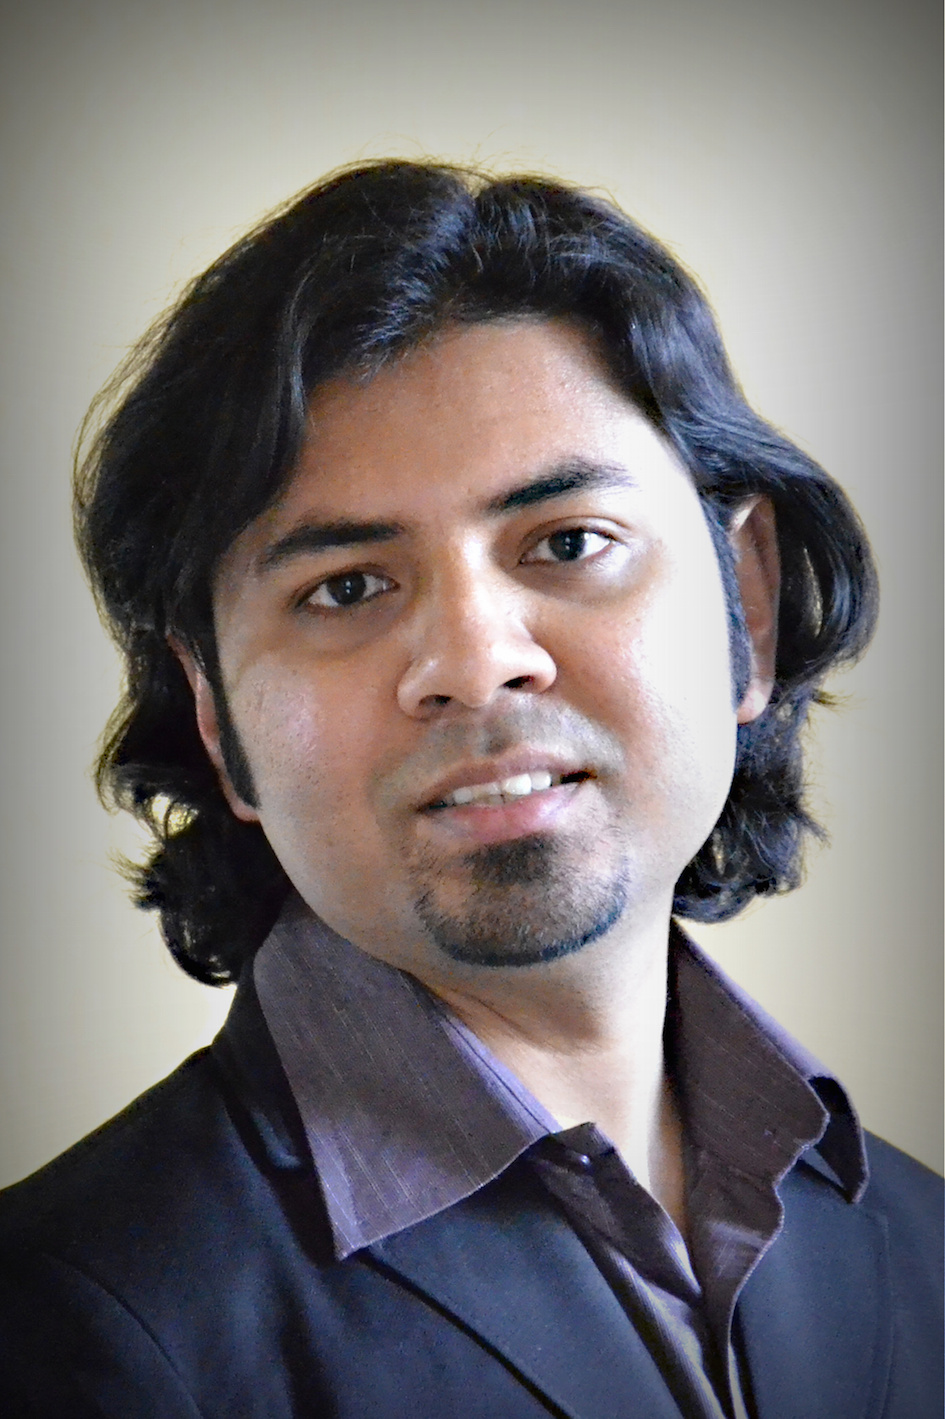
\includegraphics[width=0.25\textwidth]{Figures/Profile_photo.png}
  \end{flushright}
\end{figure}

\section{Personal Information}

\label{Personal Information}

\begin{table}[hp!]

\label{Table CV1}

\begin{tabular}{>{\raggedright\arraybackslash}p{4.0cm}>{\raggedright\arraybackslash}p{10.0cm}}

\textsc{Place and Date of Birth} \vspace{0.3cm} & \begin{tabular}{>{\raggedright\arraybackslash}p{10.0cm}}Chittagong, Bangladesh\\
27 September 1986\end{tabular}\\[0.3cm]
\textsc{Nationality} \vspace{0.3cm} & \begin{tabular}{>{\raggedright\arraybackslash}p{10.0cm}}Bangladeshi\end{tabular}\\[0.3cm]
\textsc{Address} \vspace{0.3cm} & \begin{tabular}{>{\raggedright\arraybackslash}p{11.0cm}}c/o Caroline Wahle, Bergheimerstraße 81a, 69115 Heidelberg, Germany\end{tabular}\\[0.3cm]
\textsc{Phone} \vspace{0.3cm} & \begin{tabular}{>{\raggedright\arraybackslash}p{10.0cm}}004917694629256\end{tabular}\\[0.3cm]
\textsc{E-mail} \vspace{0.3cm} & \begin{tabular}{>{\raggedright\arraybackslash}p{10.0cm}}avit.bhowmik@gmail.com\end{tabular}\\[0.3cm]
\textsc{Homepage} \vspace{0.3cm} & \begin{tabular}{>{\raggedright\arraybackslash}p{10.0cm}}\href{http://avitbhowmik.ml/}{http://avitbhowmik.ml/}\end{tabular}\\

\end{tabular}

\end{table}


\section{Education}

\label{Education}

\begin{table}[hp!]

\label{Table CV2}

\begin{tabular}{>{\raggedright\arraybackslash}p{4.0cm}>{\raggedright\arraybackslash}p{10.0cm}}

\textsc{09/2011 – present} \vspace{1.2cm} & \begin{tabular}{>{\raggedright\arraybackslash}p{10.0cm}}\textbf{Doctor of Natural Sciences}\\
Quantitative Landscape Ecology, Institute for Environmental Sciences\\
University of Koblenz-Landau, Germany\\
\textit{Dissertation: Human and ecological impacts of freshwater degradation on large scales}
\end{tabular}\\[1.2cm]
\textsc{09/2010 – 03/2012} \vspace{1.8cm} & \begin{tabular}{>{\raggedright\arraybackslash}p{10.0cm}}\textbf{Master of Science in Geospatial Technologies}\\
Erasmus Mundus, European Commission\\
Partners: 1.School of Statistics and Information Management, New University of Lisbon, Portugal, 2.Institute for Geoinformatics, University of Münster, Germany and 3.Department of Computer Languages and Systems, University of Jaume I, Spain\\
\textit{Dissertation: Evaluation of Spatial Interpolation Techniques for Mapping Climate Variables with low sample density}\end{tabular}\\[1.8cm]
\textsc{12/2004 – 10/2009} \vspace{0.5cm} & \begin{tabular}{>{\raggedright\arraybackslash}p{10.0cm}}\textbf{Bachelor of Science in Urban \& Regional Planning}\\
Department of Urban \& Regional Planning\\
Bangladesh University of Engineering \& Technology\\
\textit{Dissertation: Relocation of Hazaribagh Tannery: Myth or Reality?}\end{tabular}\\

\end{tabular}

\end{table}


\section{Research Interests}

\label{Research Interests}

\begin{table}[hp!]

\label{Table CV3}

\begin{tabular}{>{\raggedright\arraybackslash}p{14.0cm}}

Spatial Eco(toxico)logy\\[0.2cm]
Climate\\[0.2cm]
Geographic Information Science \& Systems (GIS)\\[0.2cm]
Multivariate Statistics, Spatial Statistics, Geostatistics\\

\end{tabular}

\end{table}


\section{Research Activities}

\label{Research Activities}

\begin{table}[hp!]

\label{Table CV4}

\begin{tabular}{>{\raggedright\arraybackslash}p{4.0cm}>{\raggedright\arraybackslash}p{10.0cm}}

\textsc{04/2012 – 07/2012} \vspace{1.4cm} & \begin{tabular}{>{\raggedright\arraybackslash}p{10.0cm}}\textbf{Research Assistant}\\
Institute for Geoinformatics, University of Münster, Germany\\
\textit{Responsibilities: 1. Development of online demonstrators and web tools for core concepts of spatial information, and 2. Taught courses – (i) Reference Systems for Geographic Information, (ii) Developing Demonstrators for Core Concepts of Spatial Information and (iii) Digital Cartography}\\
\end{tabular}\\[1.4cm]
\textsc{03/2008 – 10/2010} \vspace{2.6cm} & \begin{tabular}{>{\raggedright\arraybackslash}p{10.0cm}}\textbf{Project Assistant}\\
Faculty of Spatial Planning, Technical University of Dortmund, Germany\\
Project: ``The Struggle for Urban Livelihoods and the Quest for a Functional City Reconciling Informal and Statutory Planning Institutions in Dhaka, Bangladesh'', supported by German research foundation (DFG)\\
\textit{Responsibilities: 1. Preparation of Geographic Information Systems (GIS) databases, 2. Analyses and processing of empirical data, and 3. Conduction of empirical field investigation, i.e. key informant interviews, group discussion, household interviews and exercise of Venn-diagram and observations}\end{tabular}\\[2.6cm]
\textsc{12/2008 – 01/2009} \vspace{0.5cm} & \begin{tabular}{>{\raggedright\arraybackslash}p{10.0cm}}\textbf{Project Intern}\\
AQUA Consultants \& Associates, Bangladesh\\
Project: ``Preparation of Master Plan for Pourashavas under Upazilla Town Infrastructure Development''\\
\textit{Responsibilities: Digitization of cadastral maps and creation of GIS coverages}
\end{tabular}\\

\end{tabular}

\end{table}



\section{Publications}

\label{Publications}

\subsection{Peer Reviewed Journal Articles}

\label{Peer Reviewed Journal Articles}

\begin{table}[hp!]

\label{Table CV5}

\begin{tabular}{>{\raggedright\arraybackslash}p{14.0cm}}

\textbf{Bhowmik}, A.K., Alamdar, A., Katsoyiannis, I., Shen, H., Ali, N., Ali, S.M., Bokhari, H., Schäfer, R.B., Eqani, S.A.M.A.S., 2015. Mapping human health risks from exposure to trace metal contamination of drinking water sources in Pakistan. Science of The Total Environment 538, 306–316. doi:10.1016/j.scitotenv.2015.08.069\\

\end{tabular}

\end{table}

\newpage

\begin{table}[hp!]

\label{Table CV5a}

\begin{tabular}{>{\raggedright\arraybackslash}p{14.0cm}}

\textbf{Bhowmik}, A.K., Schäfer, R.B., 2015. Large Scale Relationship between Aquatic Insect Traits and Climate. PLOS ONE 10, e0130025. doi:10.1371/journal.pone.0130025\\[0.3cm]
\textbf{Bhowmik}, A.K., Metz, M., Schäfer, R.B., 2015. An automated, objective and open source tool for stream threshold selection and upstream riparian corridor delineation. Environmental Modelling & Software 63, 240–250. doi:10.1016/j.envsoft.2014.10.017\\[0.3cm]
\textbf{Bhowmik}, A.K., Costa, A.C., 2014. Representativeness impacts on accuracy and precision of climate spatial interpolation in data-scarce regions. Meteorological Applications 22, 368–377. doi:10.1002/met.1463\\[0.3cm]
\textbf{Bhowmik}, A.K., 2013. Industries’ Location as Jeopardy for Sustainable Urban Development in Asia: A Review of the Bangladesh Leather Processing Industry Relocation Plan. Environment and Urbanization Asia 4, 93–119. doi:10.1177/0975425313477749\\[0.3cm]
\textbf{Bhowmik}, A.K., Cabral, P., 2013. Cyclone Sidr Impacts on the Sundarbans Floristic Diversity. Earth Science Research 2. doi:10.5539/esr.v2n2p62\\[0.3cm]
\textbf{Bhowmik}, A.K., 2013. Temporal Patterns of the Two-Dimensional Spatial Trends in Summer Temperature and Monsoon Precipitation of Bangladesh. ISRN Atmospheric Sciences 2013, 1–16. doi:10.1155/2013/148538\\[0.3cm]
\textbf{Bhowmik}, A.K., 2012. A Geostatistical Approach to the Seasonal Precipitation Effect on Boro Rice Production in Bangladesh. International Journal of Geosciences 03, 443–462. doi:10.4236/ijg.2012.33048\\[0.3cm]
\textbf{Bhowmik}, A.K., 2012. A Comparison of Bangladesh Climate Surfaces from the Geostatistical Point of View. ISRN Meteorology 2012, 1–20. doi:10.5402/2012/353408

\end{tabular}

\end{table}


\section{Scholarships and Awards}

\label{Scholarships and Awards}

\begin{table}[hp!]

\label{Table CV6}

\begin{tabular}{>{\raggedright\arraybackslash}p{4.0cm}>{\raggedright\arraybackslash}p{10.0cm}}

%\textsc{2014} \vspace{0.7cm} & \begin{tabular}{>{\raggedright\arraybackslash}p{10.0cm}}\textbf{AGILE Early Career Scientist Grant}\\
%\textit{17th International Conference on Geographic Information Science}\\
%Castellon, Spain
%\end{tabular}\\[0.7cm]
\textsc{2013} \vspace{0.7cm} & \begin{tabular}{>{\raggedright\arraybackslash}p{10.0cm}}\textbf{CORDEX Young Scientist Award}\\
\textit{International Conference on Regional Climate - CORDEX 2013}\\
Brussels, Belgium
\end{tabular}\\[0.7cm]
\textsc{2013} \vspace{0.7cm} & \begin{tabular}{>{\raggedright\arraybackslash}p{10.0cm}}\textbf{Best paper award}\\
%\textit{Space-Time Variability of Summer Temperature Field over Bangladesh during 1948-2007}\\
\textit{13th International Conference on Computational Science and its Applications (ICCSA 2013)}, Ho Chi Minh City, Vietnam
\end{tabular}\\[0.7cm]
\textsc{2012–2015} \vspace{0.6cm} & \begin{tabular}{>{\raggedright\arraybackslash}p{10.0cm}}\textbf{Quantitative Landscape Ecology Ph.D. Scholarship}\\
%\textit{Through a German Research Foundation (DFG) grant}\\
University of Koblenz-Landau, Germany
\end{tabular}\\[0.6cm]
\textsc{2010 – 2012} \vspace{0.7cm} & \begin{tabular}{>{\raggedright\arraybackslash}p{10.0cm}}\textbf{Erasmus Mundus Scholarship}\\
%\textit{Master of Science in Geospatial Technology}\\
\textit{The Education, Audiovisual and Culture Executive Agency (EACEA)}\\
European Commission
\end{tabular}\\[0.7cm]
\textsc{2009} & \begin{tabular}{>{\raggedright\arraybackslash}p{10.0cm}}\textbf{Mitsubishi Corporation International Merit Scholarship}\\
%\textit{For excellent academic performance in bachelor’s studies}\\
Mitsubishi Corporation, Japan
\end{tabular}\\
%\textsc{2009} & \begin{tabular}{>{\raggedright\arraybackslash}p{10.0cm}}\textbf{University Grants Commission Merit Scholarship}\\
%\textit{For sound academic and extra-curricular activities}\\
%University Grants Commission of Bangladesh
%\end{tabular}\\

\end{tabular}

\end{table}